\documentclass{report}
\usepackage{graphicx}
\usepackage[utf8]{inputenc}


\begin{document}

\begin{titlepage}


\center % Center everything on the page
 

\includegraphics[width=1.0\textwidth]{img/logos.png}

\vfill % Fill the rest of the page with whitespace

\textsc{\LARGE MOLUSCE}\\[1.5cm] 
\textsc{\Large Modules for Land Use Change Evaluation}\\[0.5cm] 
\textsc{\large Quick Help}\\[0.5cm]

\vfill % Fill the rest of the page with whitespace

 
\textsc{
License\\
Except where otherwise noted, content of this work is licensed under a Creative
Commons Attribution-ShareAlike 3.0 Unported~License.
}

\end{titlepage}


\tableofcontents


\chapter{Plug-in overview}
\section{Introduction}

Open source software platforms are progressively becoming widely used in the public and private
sectors. In Geographical Information System (GIS), open source software packages such as QGIS
are actively being developed. More importantly, customization and further development is possible
since developers create specific plug-ins with flexibility.

Asia Air Survey Co., Ltd. (AAS) started to move towards open source software since 2012
becoming the first QGIS gold sponsor worldwide. Furthermore, open source software started to be
used more extensively for internal use and in international project. Alongside with these recent
changes AAS also started to develop open source solutions aiming to further extend its market.


\section{What is MOLUSCE?}
AAS released MOLUSCE (Modules for Land Use Change Evaluation) at FOSS4G 2013.
MOLUSCE is a user-friendly plug-in for QGIS 2.0 and above. MOLUSE is designed to analyse,
model and simulate land use/cover changes. The plug-in incorporates well-known algorithms,
which can be used in land use/cover change analysis, urban analysis as well as forestry applications
and projects.

MOLUSCE is well suited to:
\begin{itemize}
  \item analyse land use and forest cover changes between different time periods;
  \item model land use/cover transition potential or areas at risk of deforestation; 
  \item and simulate future land use and forest cover changes
\end{itemize}


\section{Functions}
MOLUSCE user interface offers an easy-to-use interface with specific modules and functions.
Following is a brief description of basic modules in MOLUSCE.

\paragraph{Input module}
Land use/cover maps from different epochs, biophysical and socio-economic driving factor data
such as road network, rivers, topography, population etc., are loaded in the input module.

\paragraph{Area change analysis}
Computes land use/cover changes between two time periods (T1 and T2). Land use/cover change
transition matrices as well as land use change maps are produced.

\paragraph{Modelling methods}
Four methods, namely Artificial Neural Networks (ANN), Logistic Regression (LR), Multi-Criteria
Evaluation (MCE) and Weights of Evidence (WoE) are used for modelling land use/cover change
transition potential.

\paragraph{Simulation}
Displays transition potential maps, certainty function (experimental) and simulation results. A
simulated (projected) land use/cover map is produced based on a Monte Carlo Cellular-automata
modelling approach.

\paragraph{Validation}
This sub-module incorporates Kappa statistics (standard Kappa, Kappa histogram and Kappa
location), which will be used to validate the accuracy of the simulated land use/cover maps.

\chapter{How to use MOLUSCE}

\section{Inputs}
A screenshot of \verb+Inputs+ tab is shown in Figure~\ref{fig:inputs_tab}.

\begin{figure}[h!]
\centering
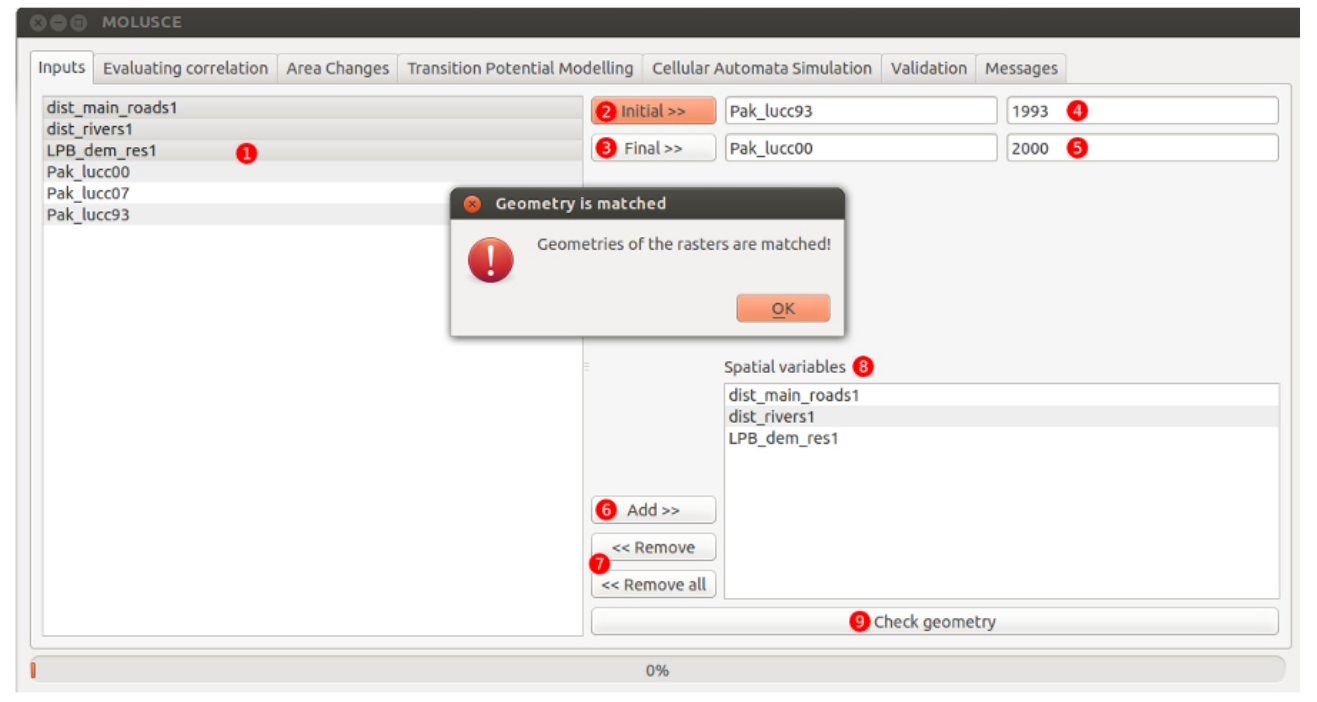
\includegraphics[width=0.95\textwidth]{img/inputs_tab.png}
\caption{Inputs tab}
\label{fig:inputs_tab}
\end{figure}

Data can be loaded using the inputs tab. To load your data follow the next steps (Figure~\ref{fig:inputs_tab}).

\begin{itemize}

  \item Step 1. Load all rasters that you need in the input tab. 
  \item Load the initial and final land use/cover maps as shown in steps 2 and 3. The base map determines
  the geometry of all the output files, pixel size, scaling and projection.
  \item Steps 4 and 5 show the corresponding years. (The user can type here If the corresponding years do
  not appear automatically).
  \item Steps 6 and 7 show how the add/remove buttons used to add or remove spatial variables.
  \item The selected spatial variables are shown in step 8.
  \item The check geometry button is a mandatory step to check if the geometry of the selected raster is
  matched (step 9).
\end{itemize}


Note: It is important when layers are added to QGIS that the No Data Value (NDV) is set. If this is
not done, MOLUSCE will process NDV areas as land use/cover classes, increasing processing time
and confusing the model calibration. MOLUSCE picks up the NDV of the input (base) layer and
propagates it to any output maps generated, along with the geometry of the base layer.

\section{Evaluating correlation}

The \verb+evaluating correlation+ module contains three techniques for performing correlation analysis:
\begin{enumerate}
  \item Pearson's correlation.
  \item Cramer's coefficient.
  \item Joint information uncertainty.
\end{enumerate}

The user can choose between a two-way raster comparison by selecting \verb+first raster+ and \verb+second raster+
or \verb+check all rasters+ loaded into MOLUSCE.

\begin{figure}[h!]
\centering
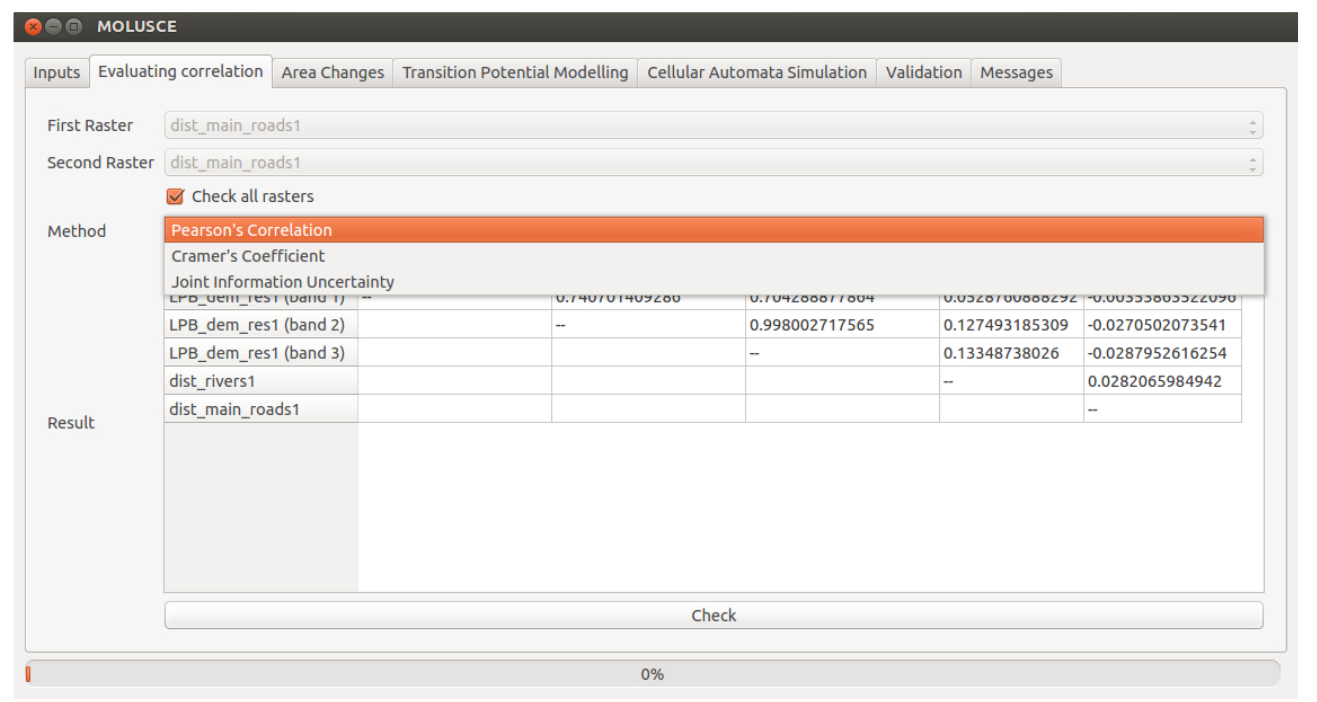
\includegraphics[width=0.95\textwidth]{img/correlation_tab.png}
\caption{Evaluation correlation tab}
\label{fig:correlation_tab}
\end{figure}

The user can run correlation by pressing the \verb+check+ button located at the bottom of the window (see Figure~\ref{fig:correlation_tab}).

Note: The \verb+Cramer's coefficient+ and \verb+joint information uncertainty+ work only with categorical data.
The data should be converted to categorical data (eg. using GRASS).

\section{Area Changes}

A screenshot of \verb+Area Changes+ tab is shown in Figure~\ref{fig:changes_tab}.

\begin{figure}[h!]
\centering
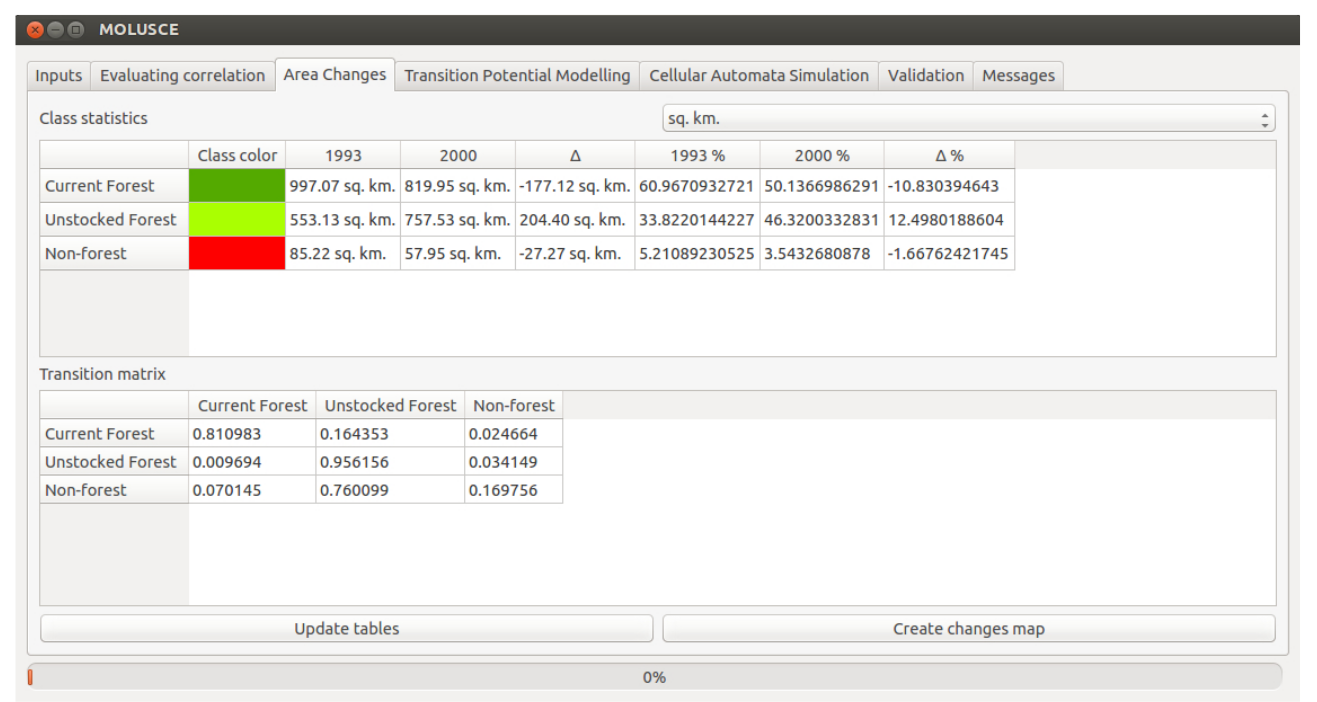
\includegraphics[width=0.95\textwidth]{img/changes_tab.png}
\caption{Area Changes tab}
\label{fig:changes_tab}
\end{figure}

The \verb+update tables+ button produces \verb+class statistics+ and \verb+transition+ \verb+matrix+ tables.

The \verb+class statistics+ table shows the initial and final land use/cover change (LUC) areas.

The \verb+transition matrix+ shows the proportions of pixels changing from one land use/cover to another.

The \verb+create change map+ button will generate a map of change classes. This will be added
automatically to QGIS and saved as a GeoTiff.

Note: Data from tables can be copied and pasted directly into spreadsheet programs, simply by
selecting the desired rows/columns and by pressing the “Ctrl~+~C” keyboard combination.

\section{Transition potential modelling}
MOLUSCE uses Artificial Neural Network (ANN), Multi Criteria Evaluation (MCE), Weights of
Evidence (WoE) and Logistic Regression (LR) methods to model land use/cover transition
potential. The user can select a \verb+method+ from the drop down menu.

ANN, WoE and LR are machine learning models; they "look" at the training samples and try 
to find patterns that are "hidden" in the samples. However MCE is different: 
it is a model in which an expert (the user) describes the importance of factors
according to his/her knowledge of the domain area. After that, the expert's knowledge is transformed into
a computational model that estimates transition potentials.




\subsection{Artificial Neural Network (ANN)}
MOLUSCE uses full-connected Multi-Layer Perceprtron for modelling.
A screenshot of an example of \verb+ANN model settings+ is shown in Figure~\ref{fig:ann_model}.

\begin{figure}[h!]
\centering
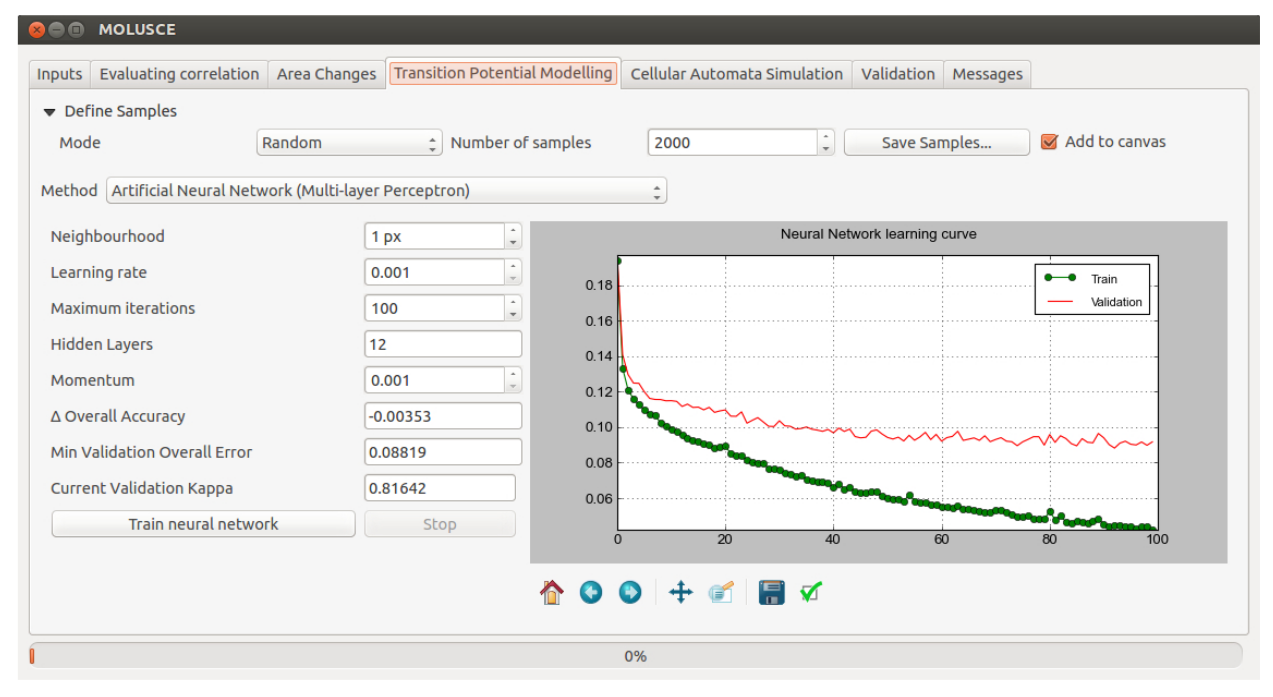
\includegraphics[width=0.95\textwidth]{img/ann_model.png}
\caption{Transition potential modelling: ANN model}
\label{fig:ann_model}
\end{figure}

The \verb+define samples+ function specify number of samples and sampling mode. In addition, the
sampling points created can be saved and displayed.

\paragraph{Inputs} Five inputs are used to customize the ANN modelling:
\begin{itemize}
  \item The \verb+neighbourhood+ defines count of neighbour pixels around current pixel. Size=1 means 9
    pixels (3x3 region), size=2 means 25 pixels (5x5), etc.
  \item \verb+Learning rate+, \verb+momentum+ and \verb+max iterations number+ define parameters of learning. Big
    learning rate and momentum allow fast learning, but the learning process can be unstable
    (spikes on the graph). Small learning rate and momentum means stable but slow learning.
  \item \verb+Hidden layers+ input string takes a list of numbers: $N_1$, $N_2$,  \dots, $N_k$, where $N_1$ is number of
    neurons in 1st hidden layer, $N_2$ is number of neurons in 2nd hidden layer and so on, $N_k$ is the
    number of neurons of the last hidden layer (k-th layer). For example if the user types in the
    input string “2” then a network with 1 hidden layer and 2 neurons will be created. In order to
    create a network with 2 hidden layers the user should insert 2 numbers, such as “10 2”
    which will create a network with 10 neurons in the first hidden layer and 2 neurons in the
    second.
\end{itemize}


\paragraph{Outputs} The following outputs are proposed (for the current learning iteration):
\begin{itemize}
  \item The graph area. Contains errors of training and validation sets. It is the main information
about learning process. The graph can be edited and saved as image.
  \item The \verb+min validation overall error+ contains information about min reached error on validation
set of samples.
  \item The \verb+delta overall accuracy+ contains difference between min reached error and current error.
  \item The \verb+current validation Kappa+ shows the Kappa value.
\end{itemize}

The training process can be started by pressing on the \verb+train neural+ \verb+network+ button and stopped at any time
using the \verb+stop+ button.

Learning algorithm analyses the reached accuracy on training and validation sets of samples and
stores the best neural net in memory. The training process finishes when the \verb+maximum iteration number+ is
reached, and the best neural net will be used to produce transition potentials.

\subsubsection{How to train the model}
There are few parameters that can dramatically change quality of trained model. 
The main of them are:
\begin{itemize}
  \item ANN complexity (number of layers and neurons): complex models are more powerfull, but training them properly is hard process, complex models require more samples to train etc. 
  \item learning rate and momentum: large values of learning rate allow to train quickly, but the training process may be unstable in this case; momentum helps stabilize the training.
  \item sample count: large sample count allows to train complex models, but the training becomes slow and requires more computer memory (which can be issue for large rasters).
\end{itemize}

So process of ANN training is a trial and error method: during the training the uses searches "good" parameters that lead to "good" model.
The training graph is the main tool that provide information about the training process and model quality.

Bellow we provie an example of ANN training, discuss some potential caveats and how to fix them.


\paragraph{Unstable learning} Figure~\ref{fig:ann_spikes} shows an example of unstable learning process: there are a lot of spikes on the graph.
Note that the learning rate is 0.1.

A stable training process is one of the necessary conditions for good ANN model: we can't expect 
to learn something usefull if the  values of its parameters show dramatic changes with every iteration.

\begin{figure}[h!]
\centering
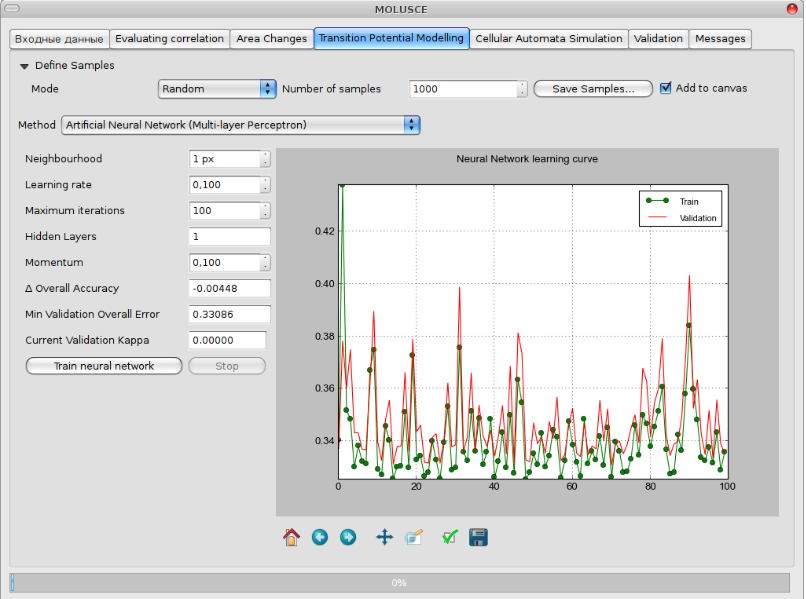
\includegraphics[width=0.95\textwidth]{img/ann_spikes.png}
\caption{ANN model: spikes on the graph (unstable training)}
\label{fig:ann_spikes}
\end{figure}

We can fix the issue if decrease the value of this parameter. Figure~\ref{fig:ann_spikes_fxd} shows 
that if we set learning rate to 0.001 the learning curves become smooth. The smooth form of 
lines for training and validation errors indicates a stable training process. This means that the
intenal values of the parameters of ANN model do not change suddenly with every iteration. 


\begin{figure}[h!]
\centering
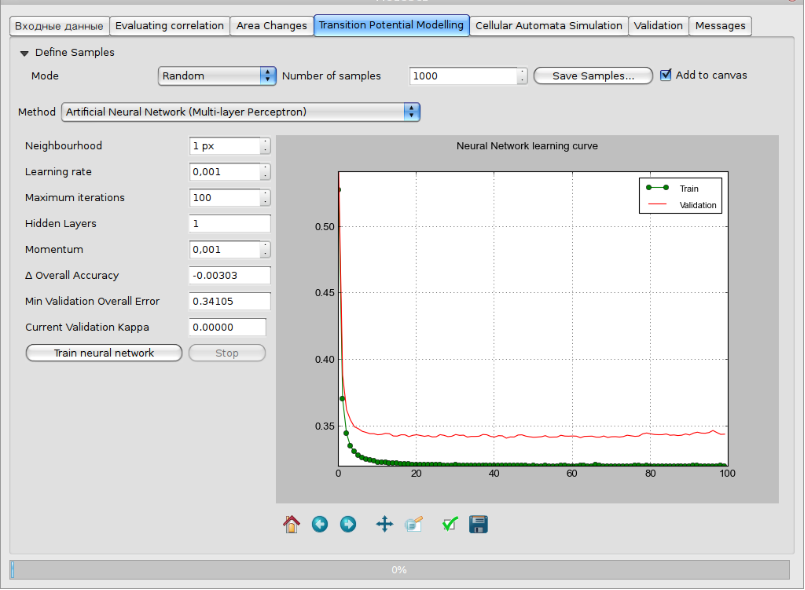
\includegraphics[width=0.95\textwidth]{img/ann_spikes_fxd.png}
\caption{ANN model: smooth learning curves}
\label{fig:ann_spikes_fxd}
\end{figure}


But we can see that the model isn't perfect (look at the Kappa and validation error).

\paragraph{Improoving the quality} Validation error and Kappa show than the model is not perfect (see Figure~\ref{fig:ann_spikes_fxd}).

We can add a neuron for the hidden layer, it makes the net more complex. The learning curves are shown in Figure~\ref{fig:ann_2neurons}.
We can see that Kappa is not zero and validation error decreases. It means that the model is getting better. 

\begin{figure}[h!]
\centering
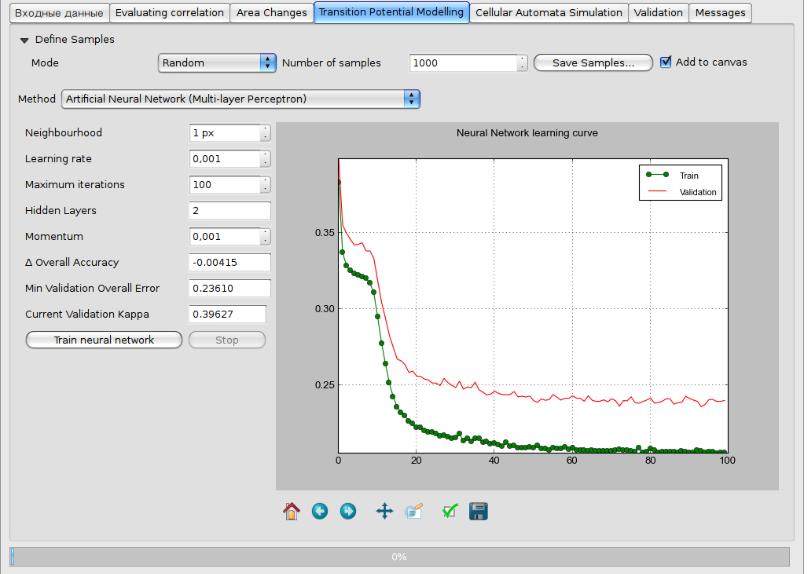
\includegraphics[width=0.95\textwidth]{img/ann_2neurons.png}
\caption{ANN model: better model with slight overfitting}
\label{fig:ann_2neurons}
\end{figure}

What about the overfitting? The model shows some overfitting (there is some difference between validation and training errors) but it is not significant.

\begin{figure}[h!]
\centering
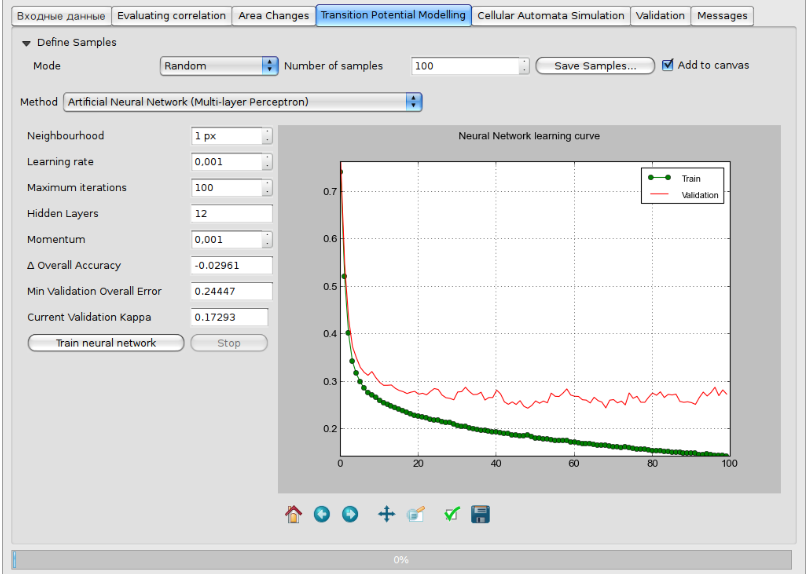
\includegraphics[width=0.95\textwidth]{img/ann_overfitting.png}
\caption{ANN model: overfitting example}
\label{fig:ann_overfitting}
\end{figure}

To get an example of clearer overfitting, set 12 neurons in the hidden layer. 
The result presented in Figure~\ref{fig:ann_overfitting}.

We can see that the trainig error is decreasing but the validation error is still nearly constant. It is clear signal about overfitting.
To avoid it we have two choices:
\begin{itemize}
    \item decrease number of neurons;
    \item increase sample count.
\end{itemize}

Figure~\ref{fig:ann_final} shows training on 20,000 samples.

\begin{figure}[h!]
\centering
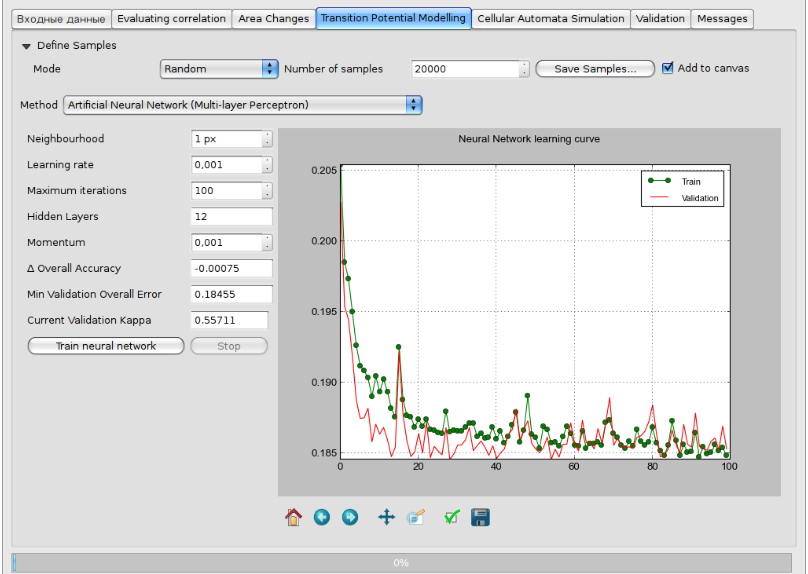
\includegraphics[width=0.95\textwidth]{img/ann_final.png}
\caption{ANN model: final example}
\label{fig:ann_final}
\end{figure}

We can see that the training and validation errors are close. Overfitting is not present.

\subsection{Multi Criteria Evaluation (MCE)}

The MCE model \cite{eastman1999multi} takes into account the expert point of view regarding the importance of the predictors. 
The user makes pairwise comparisons of the factors and describes their importance for the transition potentials. 
The comparisons are made using Saaty's scale (see~Table~\ref{tab:saaty_scale}).

\begin{table}
\centering
\caption{Saaty's scale}
\begin{tabular}{ll}
 \bf{Rating} & \bf{Preference}   \\
 1 & Equal importance  \\
 3 & Moderate importance \\ 
 5 & Strong importance \\
 7 & Very strong importance \\
 9 & Extreme importance \\
 2, 4, 6, 8 & Intermediate values 
\end{tabular}
\label{tab:saaty_scale}
\end{table}

For example, coefficient "1" between factors $A$ and $B$ means that the factors have equal importance for the transition process. 
Coefficient "9" between factors $A$ and $B$ means that factor $A$ absolutely exceeds factor $B$ in importance.

\begin{figure}[h!]
\centering
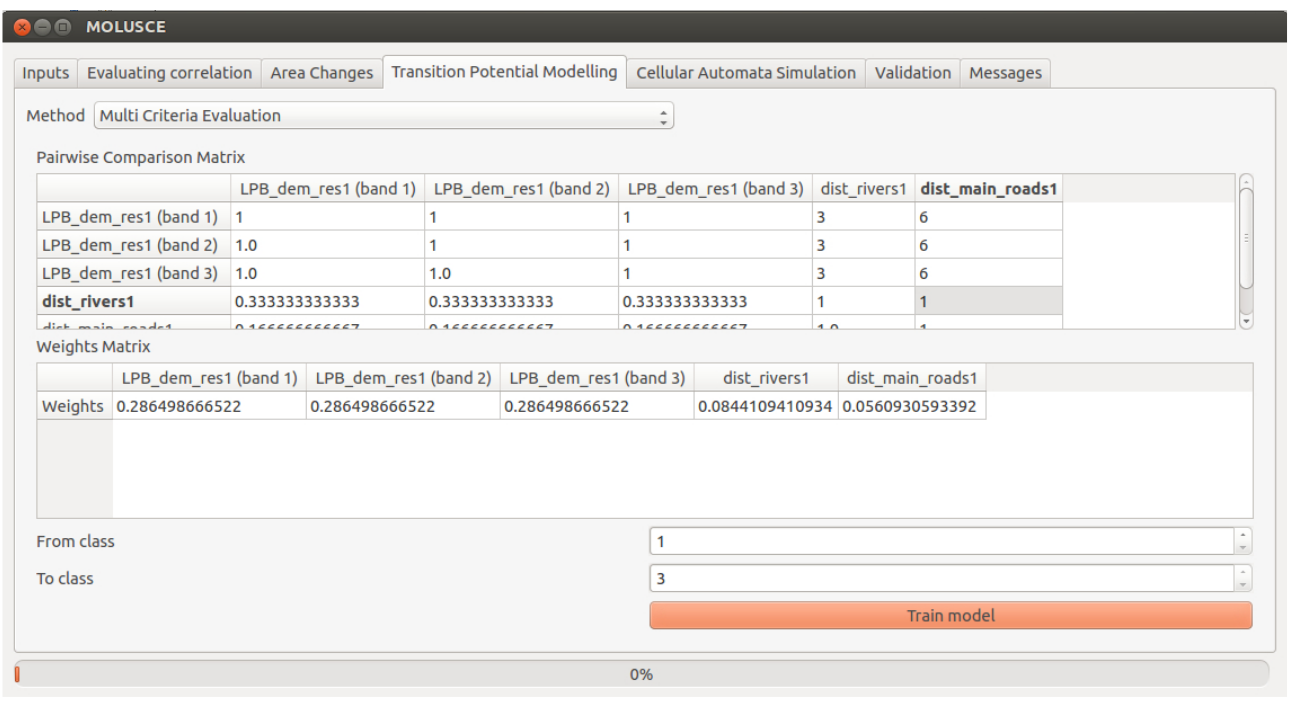
\includegraphics[width=0.95\textwidth]{img/mce_model.png}
\caption{Transition potential modelling: MCE model}
\label{fig:mce_model}
\end{figure}

A screenshot of an example of \verb+MCE model settings+ is shown in Figure~\ref{fig:mce_model}.

The user can set the values inside the \verb+pairwise comparison matrix+. 

The user can also select which classes to use to train the model by changing the \verb+from class+ 
and \verb+to class+ values located at the bottom of the window.


The model can be started by pressing the \verb+train model+ button.

The weights of the spatial variable will then appear in the \verb+weights matrix+.


\subsection{Weights of Evidence (WoE)}
The WoE \cite{bonham1989weights} method proposes two ways of defining the range breaks. 
The user can define a \verb+number of intervals+ or specify the 
\verb+range breaks+ values.

When the \verb+calculate range breaks+ button is pressed the weights information for each transition are
produced.

Once the user is satisfied with the weights the \verb+train model+ button can then be pressed.

\begin{figure}[h!]
\centering
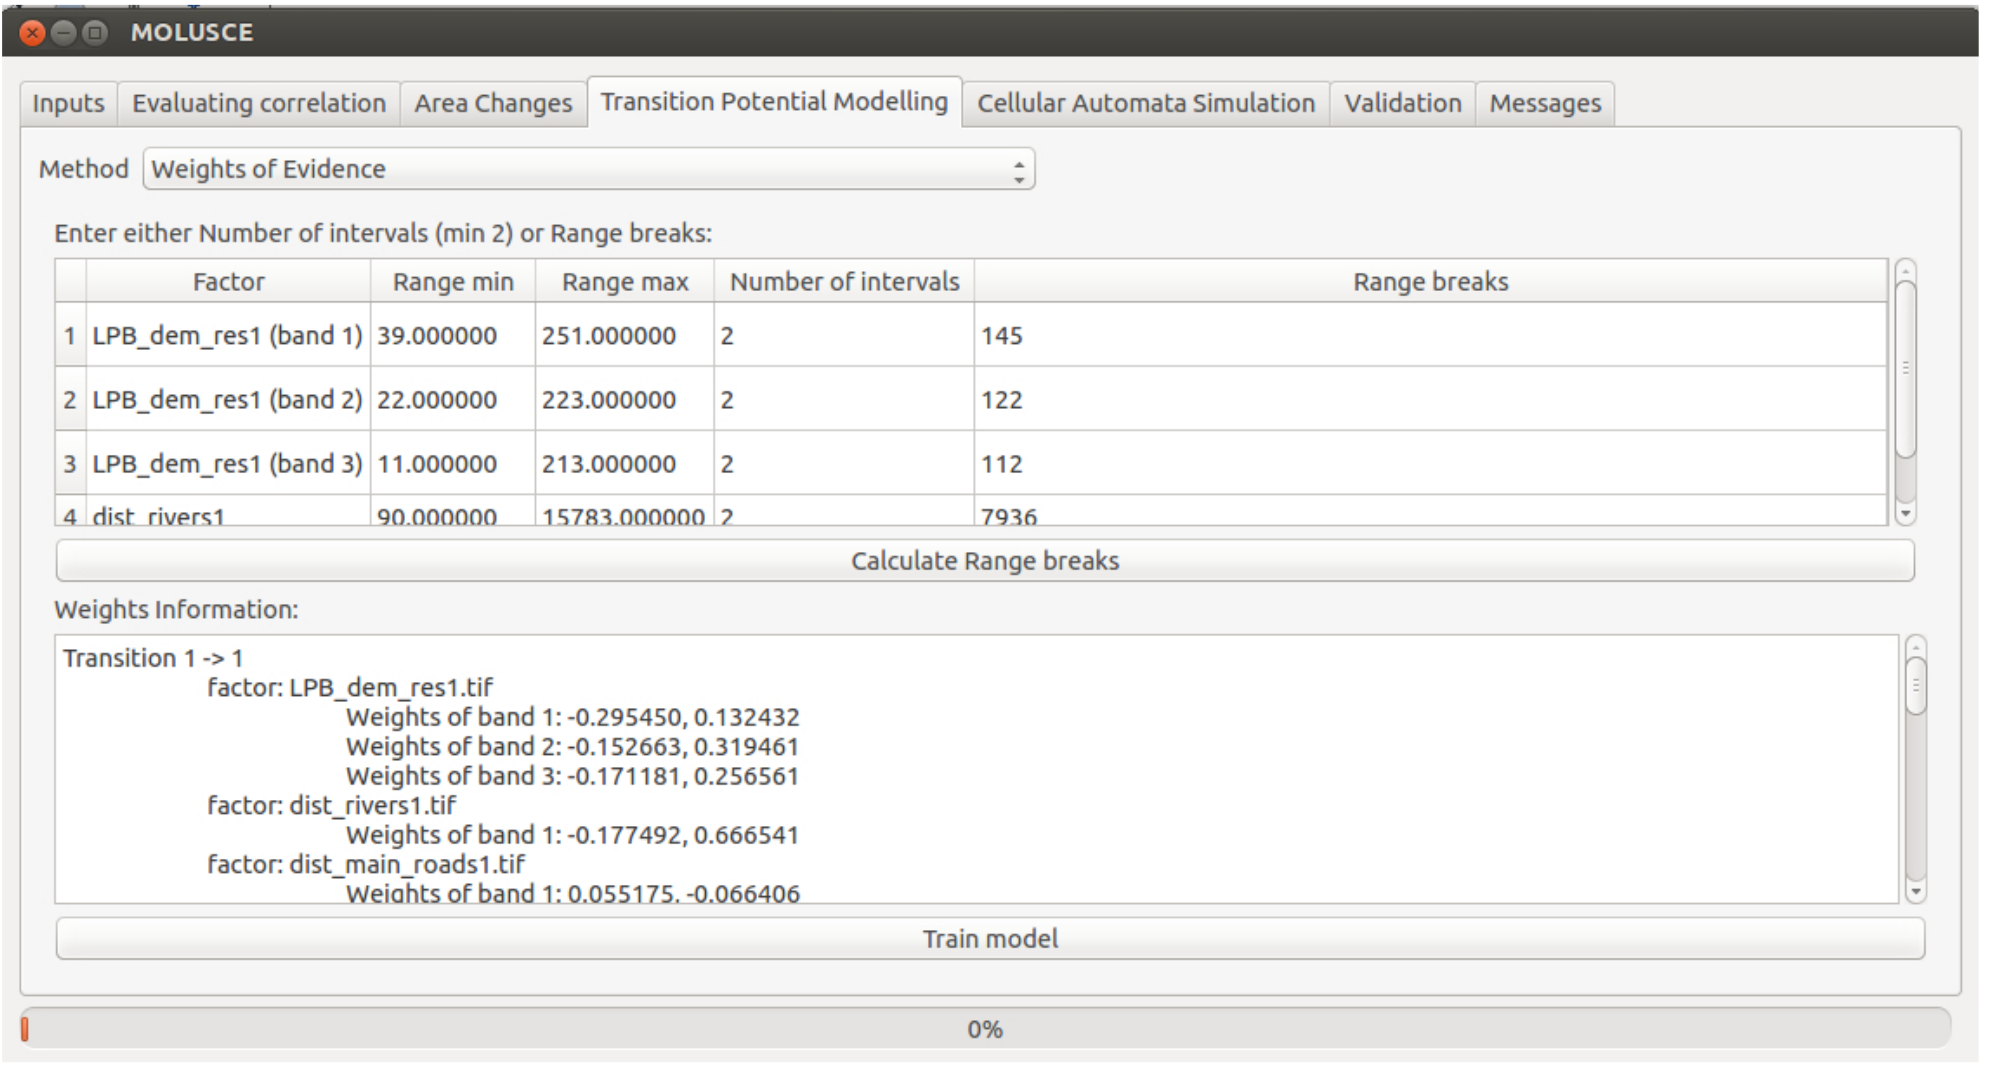
\includegraphics[width=0.95\textwidth]{img/woe_model.png}
\caption{Transition potential modelling: WOE model}
\label{fig:woe_model}
\end{figure}

An example of WoE model settings is shown in Figure~\ref{fig:woe_model}.

\subsection{Logistic Regression (LR)}

An example of LR model settings is shown in Figure~\ref{fig:lr_model}.

\begin{figure}[h!]
\centering
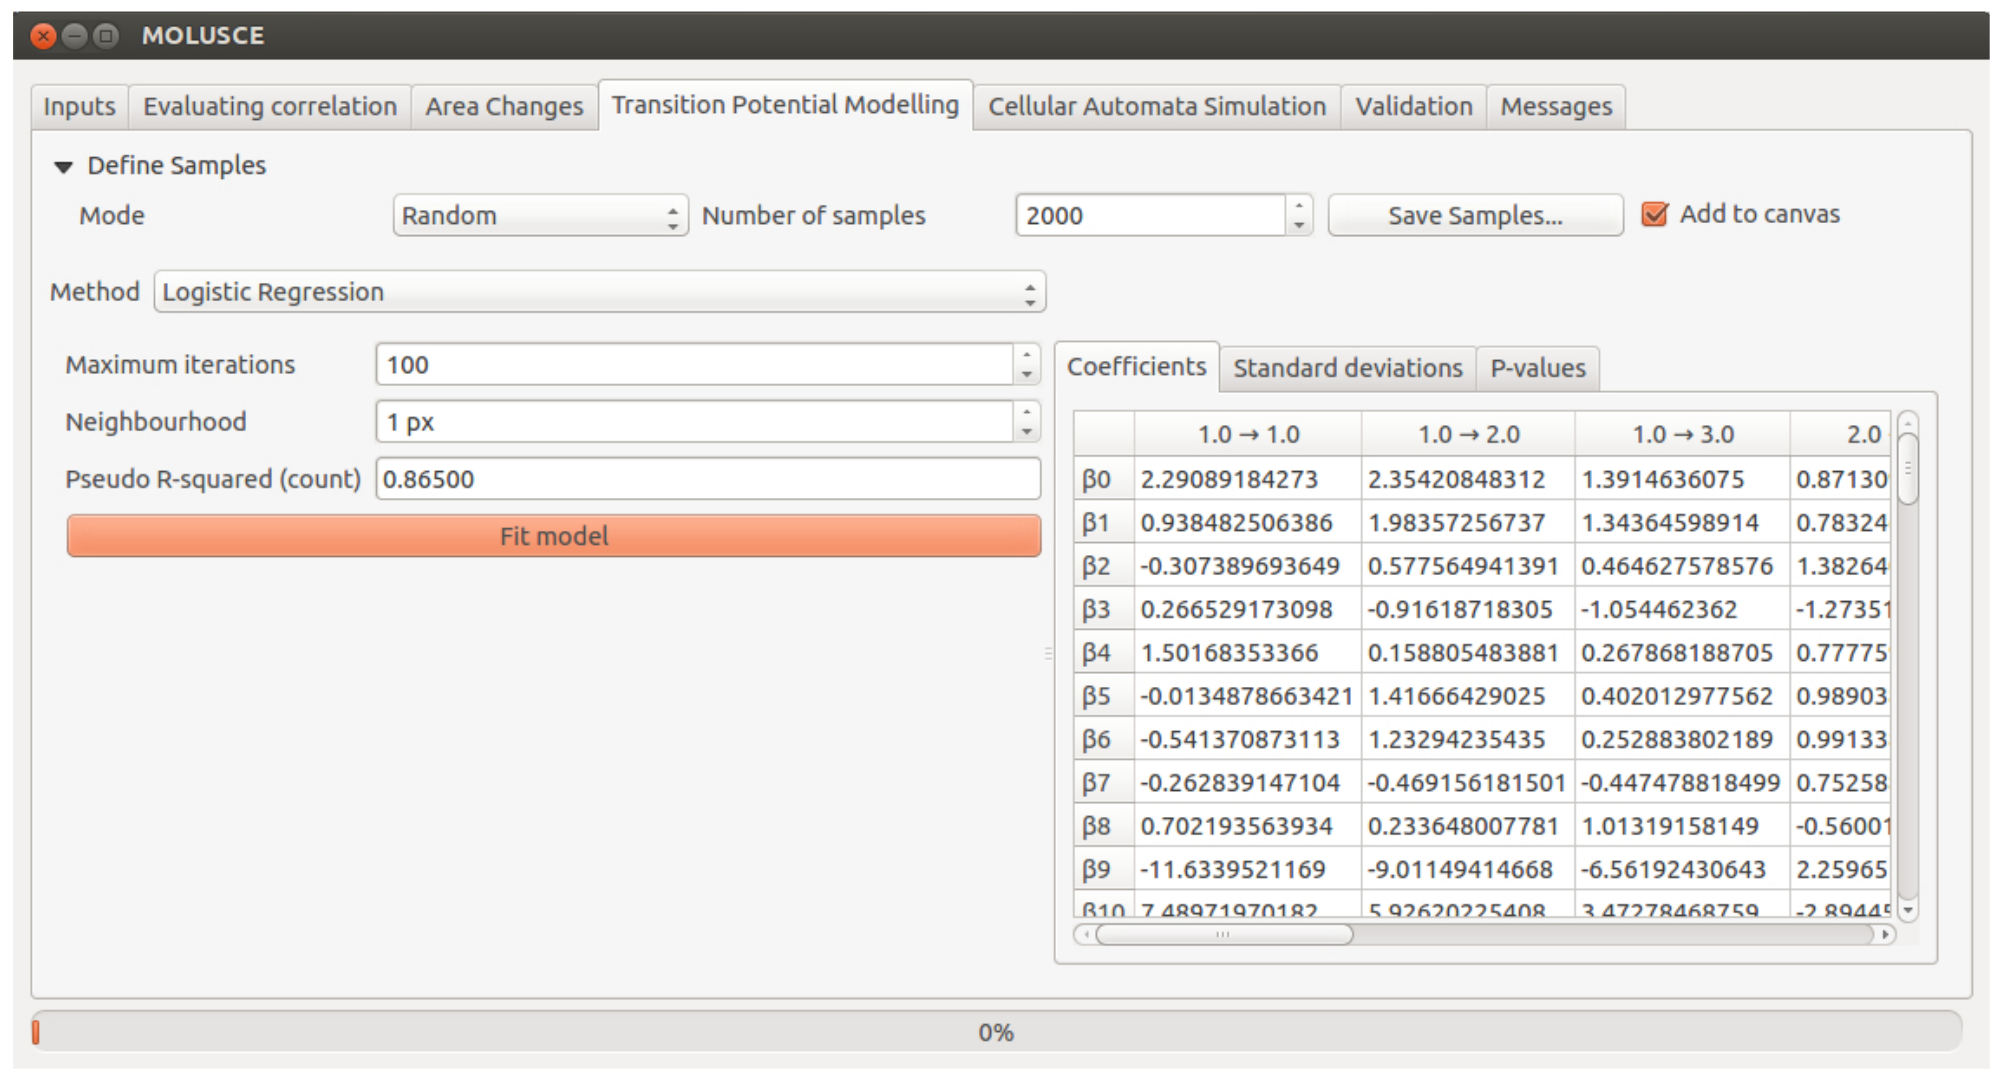
\includegraphics[width=0.95\textwidth]{img/lr_model.png}
\caption{Transition potential modelling: LR model}
\label{fig:lr_model}
\end{figure}

The LR method offers the possibility to \verb+define samples+ (number of samples and sampling mode) as
well as save and display the sampling points created.

\paragraph{Inputs} Two inputs are used to customize the LR modelling:
\begin{itemize}
  \item The \verb+maximum iteration+ defines the total number of iterations.
  \item The \verb+neighbourhood+ defines count of neighbour pixels around current pixel. Size=1 means 9
pixels (3x3 region), size=2 means 25 pixels (5x5), etc.
\end{itemize}

\paragraph{Outputs} 

The following outputs are proposed (for the current learning iteration):

\begin{itemize}
  \item The \verb+pseudo R-squared+ shows the goodness-of-fit.
  \item The \verb+coefficients+ tab.
  \item The \verb+standard deviations+ tab.
  \item The \verb+p-values+ tab.
\end{itemize}

The user can run the model by pressing on the \verb+fit model+ button.

Note: For additional information on the LR outputs please consult the “Technical information:
Methods and Algorithms” manual.


\section{Cellular Automata Simulation}

Once one method has been chosen and trained from the \verb+transition potential+ modelling tab, 
the user can then access to the \verb+cellular automata+ simulation tab.

\emph{Be aware that MOLUSCE will keep in memory the
latest method processed, if for example the user runs first the ANN and then the LR methods, the
cellular automata simulation tab will retain the results from the LR.}


\begin{figure}[h!]
\centering
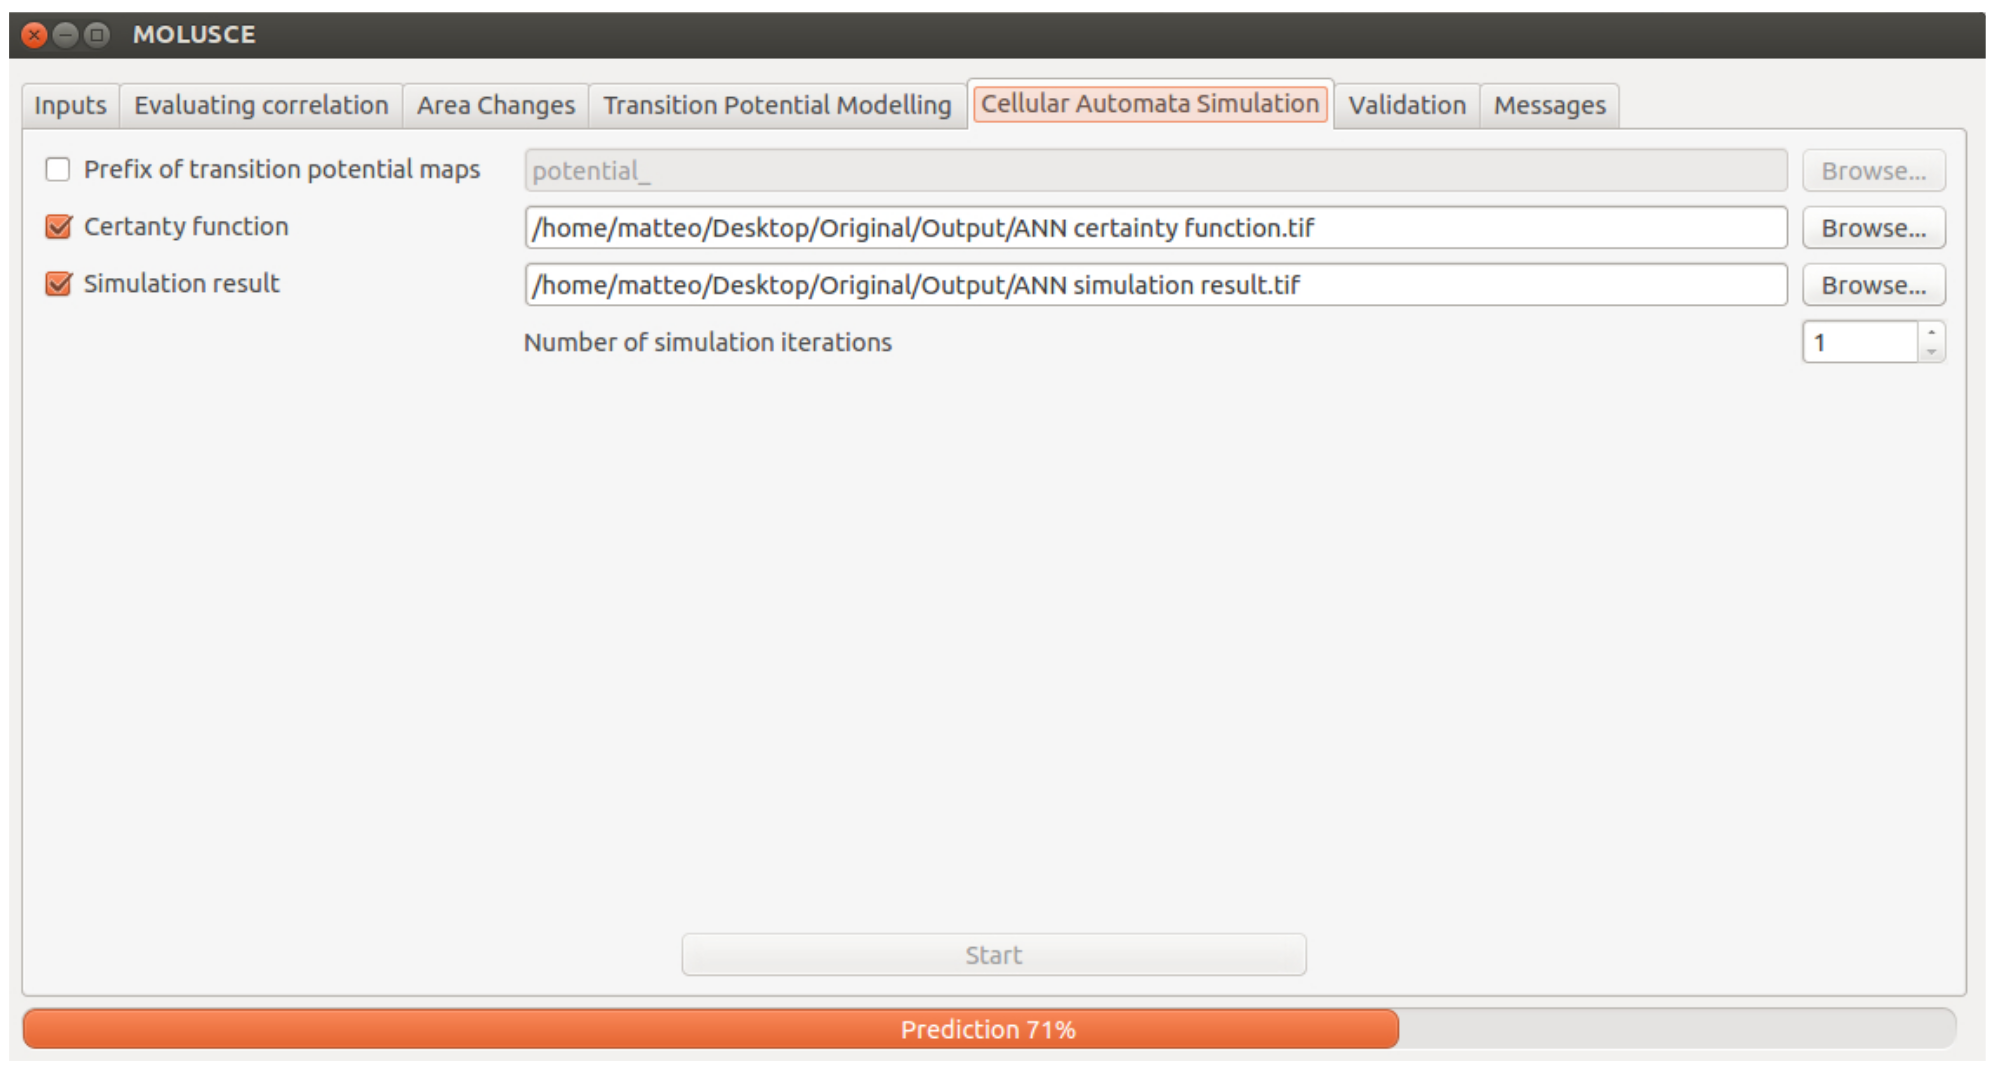
\includegraphics[width=0.95\textwidth]{img/simulation_tab.png}
\caption{Simulation tab}
\label{fig:simulation_tab}
\end{figure}

Three type of output maps are produced. A check box at the beginning of each output is provided to
allow the user to enable only what it is necessary. A \verb+browse...+ button located at the end of each
output allows to save each map.

\begin{itemize}
  \item The \verb+prefix of transition potential maps+ button allows to select prefix of the names of
    transition potential maps. Transition potential map shows the probability or potential to
    change from one land use/cover class to another. Transition potential values range from 0
    (low transition potential of change) 100 (high transition potential). Transition potential maps
    will be produced from the corresponding land use/cover changes (e.g., “forest to unstocked
    forest” transition potential, “forest to non-forest transition potential).
  \item The \verb+certainty function+.
  \item The \verb+simulation result+ produces a simulated land use/cover map.
\end{itemize}

An example of simulation tab is shown in Figure~\ref{fig:simulation_tab}.

\section{Validation}

The \verb+validation+ tab allows the user to check, validate and compare the simulation results. 
\verb+Reference+ and \verb+simulated land use/cover maps+ must be loaded in order 
to start the validation process. The
former indicates a land use/cover map ($T_3$). $T_1$ refers to the initial land use/cover, while $T_2$ refers to
the final land use/cover used in the model). A \verb+browse+ button located at the end of each output
allows to load the desired map. A two way map comparison is performed from reference land
use/cover ($T_3$) and simulated land use/cover maps.

In order to perform a three way map comparison, the user can check the \verb+risk class validation map+
check-box. Although it is not shown explicitly, the three-way map comparison uses the initial land
use/cover map ($T_1$), the reference land use/cover map ($T_3$) and the simulated land use/cover map.

The \verb+multiple-resolution budget+ method~\cite[Chapter~17]{pontius2004maps_aggreament} is also used in MOLUSCE. The user can decide the 
\verb+number of validation iterations+ and can start the process by pressing the \verb+start validation button+.
The graph can be edited and saved as image.

The overall accuracy (\verb+% of correctness+, \verb+Kappa (overall)+, \verb+Kappa (histo)+ and \verb+Kappa (loc)+) can be
executed by clicking the \verb+calculate Kappa+ button.

\begin{figure}[h!]
\centering
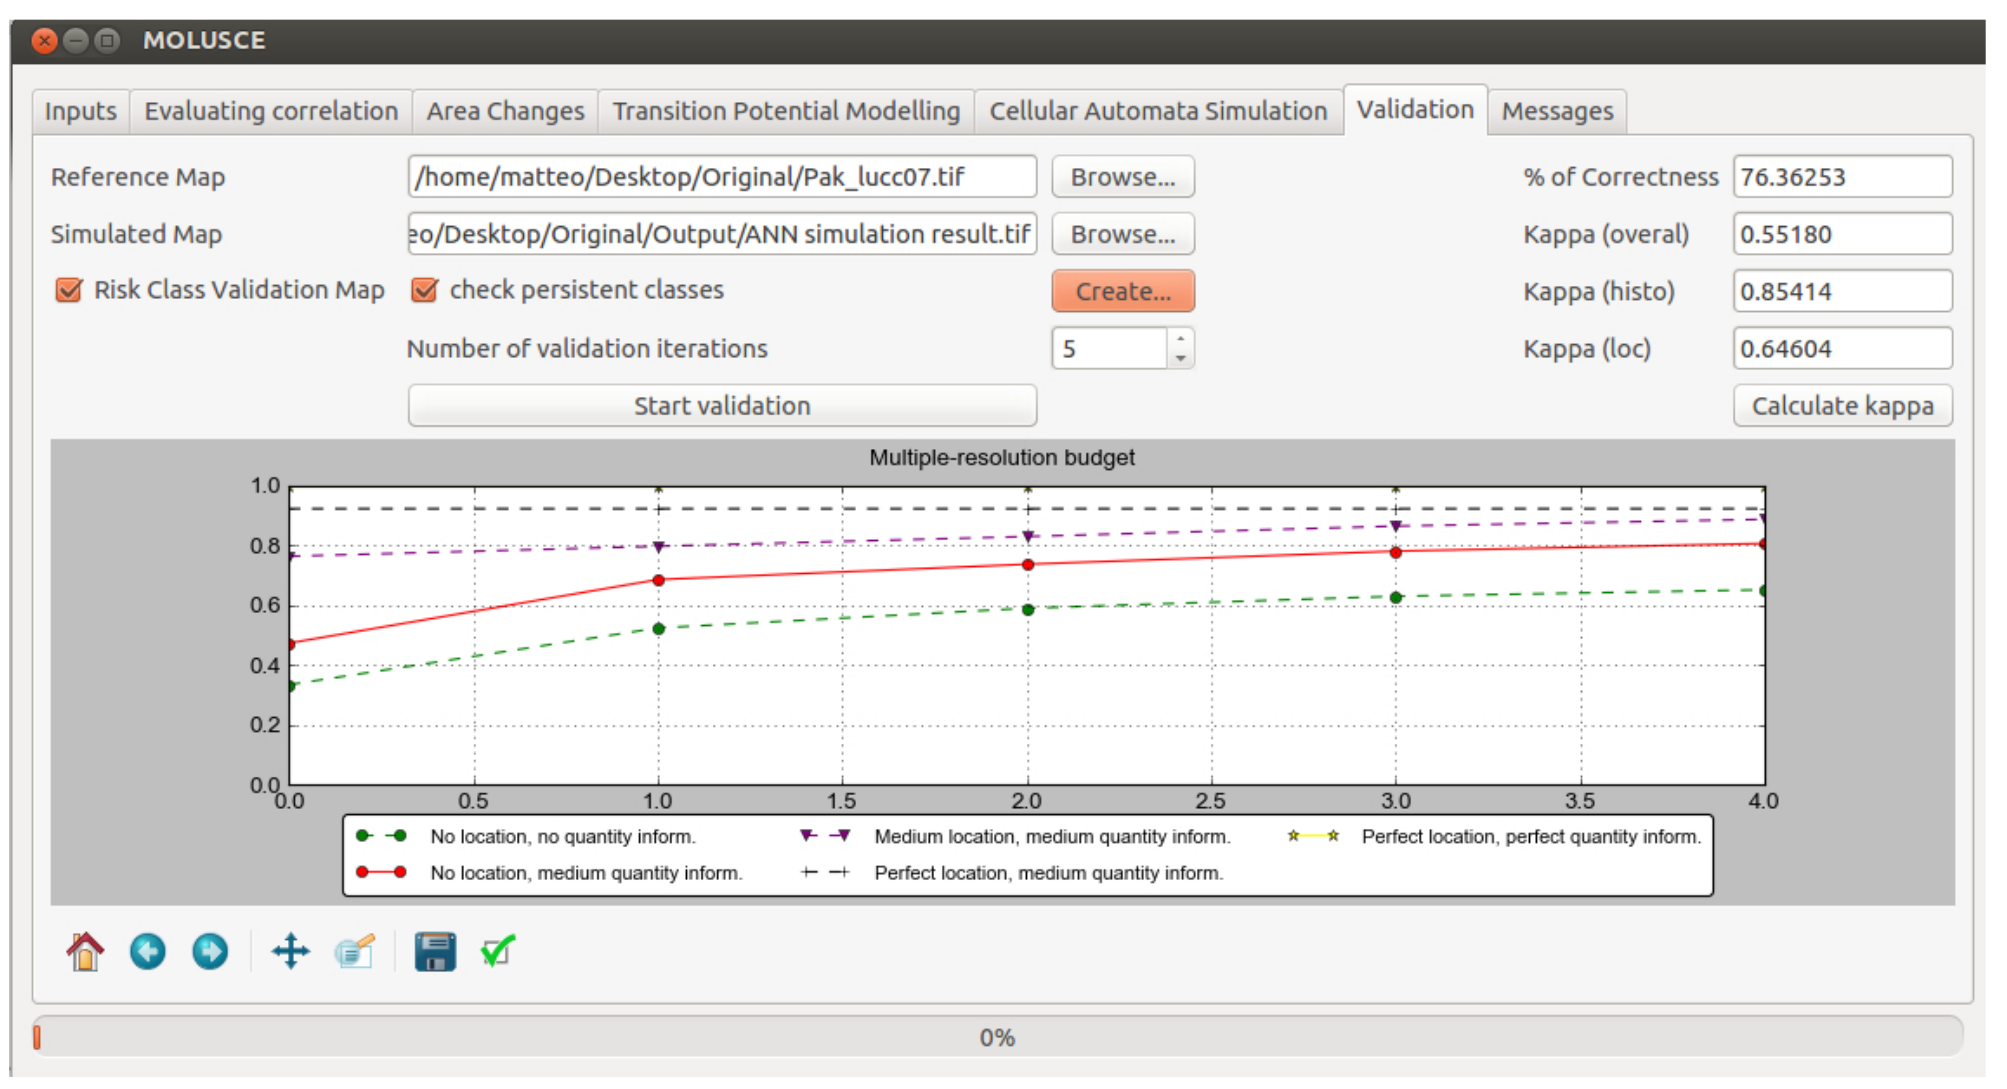
\includegraphics[width=0.95\textwidth]{img/validation_tab.png}
\caption{Validation tab}
\label{fig:validation_tab}
\end{figure}

An example of validation tab is shown in Figure~\ref{fig:validation_tab}.
We discuss here some parts of the graph, see full details in~\cite[Chapter~17]{pontius2004maps_aggreament}.
The chapter propose 15 types of statistic, but MOLUSCE calculates and plots 5 of the most important of them:
\begin{itemize}
  \item No location information, no quantity information;
  \item No location information, medium quantity information;
  \item Medium location information, medium quantity information;
  \item Perfect location information, medium quantity information;
  \item Perfect location information, perfect quantity information.
\end{itemize}

These lines aggreement metrics. They are measured for maps at different scales. 
The zero point on the abscissa axis corresponds to
the original scale of the maps, the point one corresponds the maps scaled down by half ($2^1$), the point
two corresponds the maps scaled down by quarter ($2^2$), etc.

Medium location information, medium quantity information is "the main" line.
It represents sequence of measures of agreement between the reference map and the simulated map.
Higher values of tne line show higer aggreement.

Other lines show  measures of agreement between the reference map and thouse that describe different hypothetical situations.
For example the line "No location information, no quantity information"  is the agreement due to chance.
Usually it lies below the "Medium-Medium" line, in this case the simulated map has better aggreement with the reference 
then random generated map.

The upper line, "Perfect-Perfect," represents the highest possible agreement.
It corresponds to the case when we have complete information about the reference map in advance 
and can place all changes in their correct locations during the simulation.
Thus, this line shows the case when no errors are committed.
Usually the "Medium-Medium" line lies below this line.

Other lines represents other hypothetical situations when we know more or less information
about the reference map. This information consists of two parts: infomation about the quantity of pixels (quantity of changes in our case)
and information about the locations of changes.







\bibliographystyle{plain}
\bibliography{references}

\end{document}

